{\color{bleu}\chapter{Implémentation de la Solution Proposée}}
\thispagestyle{empty}
\newpage

% =========================
% Packages needed in preamble
% =========================
% \usepackage{float}
% \usepackage{xcolor}
% \usepackage{graphicx}
% \usepackage{caption}
% \usepackage{listings}
%
% \definecolor{codebg}{RGB}{245,245,244}
% \definecolor{codeframe}{RGB}{210,210,210}
% \definecolor{codecomment}{RGB}{0,128,0}
% \definecolor{codekeyword}{RGB}{0,0,180}
% \definecolor{codestring}{RGB}{163,21,21}
%
% \lstdefinestyle{sonacode}{
%     backgroundcolor=\color{codebg},
%     frame=single,
%     rulecolor=\color{codeframe},
%     basicstyle=\ttfamily\small,
%     keywordstyle=\color{codekeyword}\bfseries,
%     commentstyle=\color{codecomment},
%     stringstyle=\color{codestring},
%     breaklines=true,
%     showstringspaces=false,
%     tabsize=2,
%     captionpos=b
% }

{\color{bleu} \section{Introduction}}

\par Ce chapitre présente la mise en œuvre concrète de la solution proposée dans le chapitre précédent. L’objectif est de montrer les étapes réelles de déploiement de l’infrastructure hyperconvergée, depuis l’installation de la plateforme de virtualisation jusqu’aux services applicatifs et aux mécanismes d’automatisation. Pour améliorer la lisibilité, l’implémentation est organisée en trois grandes parties : la couche calcul, la couche stockage, puis la couche réseau.\\

\par Les opérations ont été réalisées avec plusieurs outils complémentaires : l’interface web Proxmox VE, la ligne de commande Linux, les fichiers de configuration système, OPNsense, Ceph, ainsi que des playbooks Ansible pour automatiser certaines tâches répétitives. Des captures d’écran sont prévues aux points importants afin d’illustrer visuellement les résultats obtenus.\\

{\color{bleu} \section{Partie I --- Couche Calcul}}

{\color{bleuu} \subsection{Préparation de l’Infrastructure Physique}}

{\color{bleuuu} \subsubsection{Installation de Proxmox VE sur les nœuds}}

\par L’installation de la plateforme de virtualisation a commencé par le téléchargement de l’image ISO de Proxmox VE version 9.1.1. Cette image a ensuite été copiée sur une clé USB bootable utilisée pour démarrer chaque serveur Dell PowerEdge R720. Une installation séparée a été réalisée sur chacun des trois nœuds du cluster.\\

\par Pendant l’installation, le disque système \texttt{sda} a été utilisé pour héberger Proxmox VE. Une configuration réseau statique a aussi été appliquée afin de donner à chaque nœud une adresse de management fixe sur le réseau physique \texttt{192.168.10.0/24}. Les adresses retenues sont \texttt{192.168.10.100} pour PVE-01, \texttt{192.168.10.213} pour PVE-02 et \texttt{192.168.10.84} pour PVE-03.\\

\par Une fois l’installation terminée, la vérification a été effectuée à travers l’interface web de Proxmox, accessible sur le port \texttt{8006}. Cette étape a permis de confirmer que chaque nœud était opérationnel et prêt pour la suite du déploiement.\\

\begin{figure}[H]
    \centering
    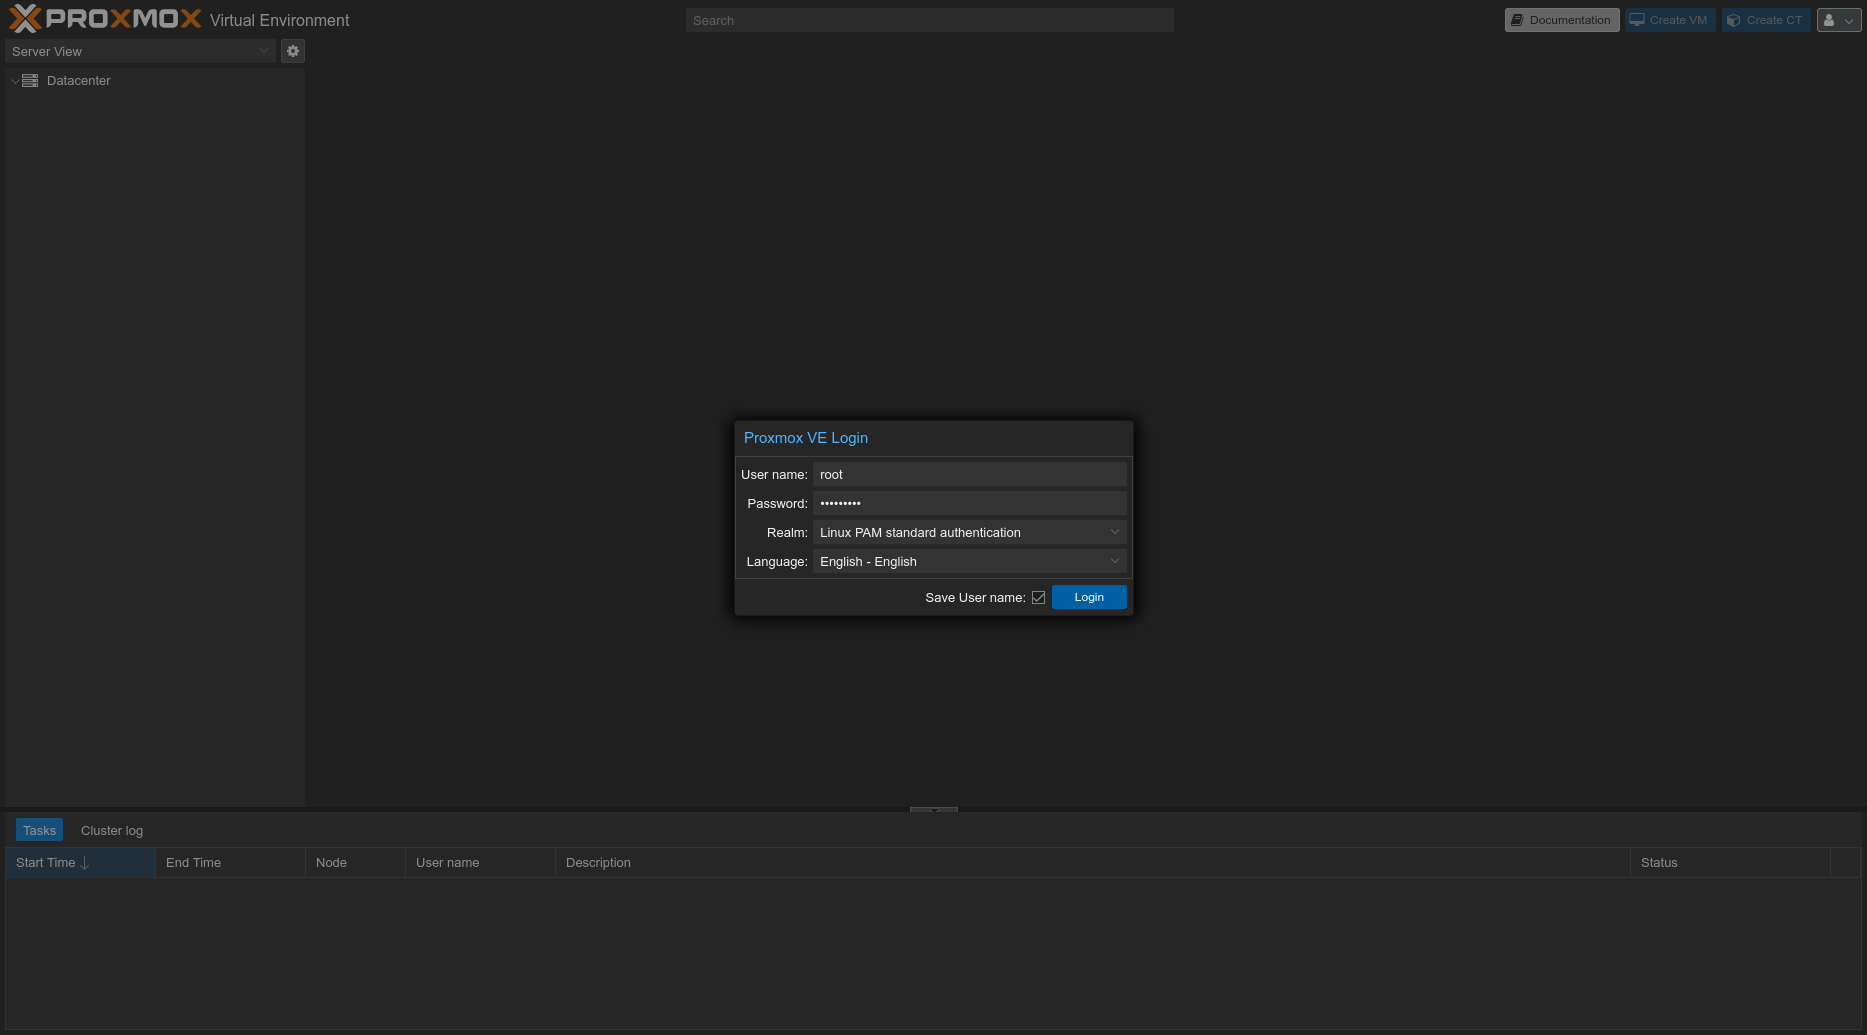
\includegraphics[width=0.9\textwidth]{image/ch4/proxmox.png}
    \caption{Interface web Proxmox au premier login sur PVE-01}
    \label{fig:proxmox-first-login}
\end{figure}

{\color{bleuuu} \subsubsection{Configuration de la connectivité Internet via le laptop gateway}}

\par Dans l’environnement de laboratoire, aucun routeur physique dédié n’était disponible pour fournir l’accès Internet aux nœuds Proxmox. Pour cette raison, un laptop a été configuré pour jouer le rôle de passerelle NAT entre le réseau interne de l’infrastructure et Internet. Il possède deux interfaces : \texttt{enp0s20f0u4c2} côté infrastructure avec l’adresse \texttt{192.168.10.36/24}, et \texttt{wlan0} côté Internet avec l’adresse \texttt{10.247.78.8/24}.\\

\par La première étape consiste à activer le routage IP afin que le système puisse transférer les paquets d’une interface à l’autre. Cette activation doit être faite de manière immédiate puis rendue permanente.\\

\begin{lstlisting}[style=sonacode,language=bash,caption={Activation du routage IP sur le laptop},label={lst:ipforward}]
sudo sysctl -w net.ipv4.ip_forward=1
sudo vim /etc/sysctl.d/99-ipforward.conf
# Ajouter :
net.ipv4.ip_forward=1
\end{lstlisting}

\par Ensuite, des règles \texttt{iptables} ont été ajoutées pour réaliser la translation d’adresses NAT et autoriser le forwarding du trafic entre les interfaces du laptop.\\

\begin{lstlisting}[style=sonacode,language=bash,caption={Configuration NAT avec iptables},label={lst:iptables-nat}]
sudo iptables -t nat -A POSTROUTING -o wlan0 -j MASQUERADE
sudo iptables -A FORWARD -i enp0s20f0u4c2 -o wlan0 -j ACCEPT
sudo iptables -A FORWARD -i wlan0 -o enp0s20f0u4c2 -m state --state RELATED,ESTABLISHED -j ACCEPT
\end{lstlisting}

\par Pour éviter de perdre ces règles après redémarrage, elles ont été sauvegardées puis activées automatiquement au boot du laptop.\\

\begin{lstlisting}[style=sonacode,language=bash,caption={Persistance des règles iptables},label={lst:iptables-persist}]
sudo pacman -S iptables-nft
sudo iptables-save | sudo tee /etc/iptables/iptables.rules
sudo systemctl enable iptables
\end{lstlisting}

\par Sur chaque nœud Proxmox, la passerelle par défaut a été définie vers \texttt{192.168.10.36}, avec des serveurs DNS publics. Cette configuration a été ajoutée dans le fichier \texttt{/etc/network/interfaces}.\\

\begin{lstlisting}[style=sonacode,language={},caption={Configuration réseau de base d’un nœud Proxmox},label={lst:proxmox-basic-network}]
auto vmbr0
iface vmbr0 inet static
    address 192.168.10.XX/24
    gateway 192.168.10.36
    dns-nameservers 8.8.8.8 8.8.4.4
\end{lstlisting}

\par Enfin, des routes statiques ont été ajoutées sur le laptop afin de rediriger les réseaux internes \texttt{172.16.60.0/24}, \texttt{172.16.70.0/24} et \texttt{172.16.80.0/24} vers la VM OPNsense, qui assure ensuite le routage vers ces sous-réseaux.\\

\begin{lstlisting}[style=sonacode,language=bash,caption={Ajout des routes statiques vers OPNsense},label={lst:static-routes-opnsense}]
nmcli connection modify "Wired connection 1" \
 +ipv4.routes "172.16.60.0/24 192.168.10.65" \
 +ipv4.routes "172.16.70.0/24 192.168.10.65" \
 +ipv4.routes "172.16.80.0/24 192.168.10.65"

nmcli connection up "Wired connection 1"
\end{lstlisting}

\par Des tests simples comme \texttt{ping 8.8.8.8}, \texttt{ping google.com} et \texttt{apt update} ont confirmé que les nœuds disposaient correctement d’un accès Internet.\\

{\color{bleuu} \subsection{Formation du cluster Proxmox et haute disponibilité}}

{\color{bleuuu} \subsubsection{Création et jonction au cluster}}

\par Après l’installation de Proxmox VE sur les trois serveurs, la phase suivante a consisté à former un cluster unique. Cette opération a été lancée depuis le premier nœud PVE-01, qui devient le nœud initial du cluster.\\

\begin{lstlisting}[style=sonacode,language=bash,caption={Création du cluster Proxmox},label={lst:pvecm-create}]
pvecm create Cluster-Proxmox-VE
\end{lstlisting}

\par Les deux autres nœuds ont ensuite rejoint ce cluster en utilisant l’adresse IP du nœud principal.\\

\begin{lstlisting}[style=sonacode,language=bash,caption={Jonction de PVE-02 et PVE-03 au cluster},label={lst:pvecm-add}]
pvecm add 192.168.10.100
\end{lstlisting}

\par Le réseau Corosync, utilisé pour le heartbeat entre les nœuds, a été isolé sur le VxLAN 20 afin de séparer le trafic de cluster du reste du trafic d’administration ou de production. Une fois la configuration terminée, la commande de vérification a confirmé la présence des trois nœuds avec quorum atteint.\\

\begin{lstlisting}[style=sonacode,language=bash,caption={Vérification de l’état du cluster},label={lst:pvecm-status}]
pvecm status
\end{lstlisting}

\begin{figure}[H]
    \centering
    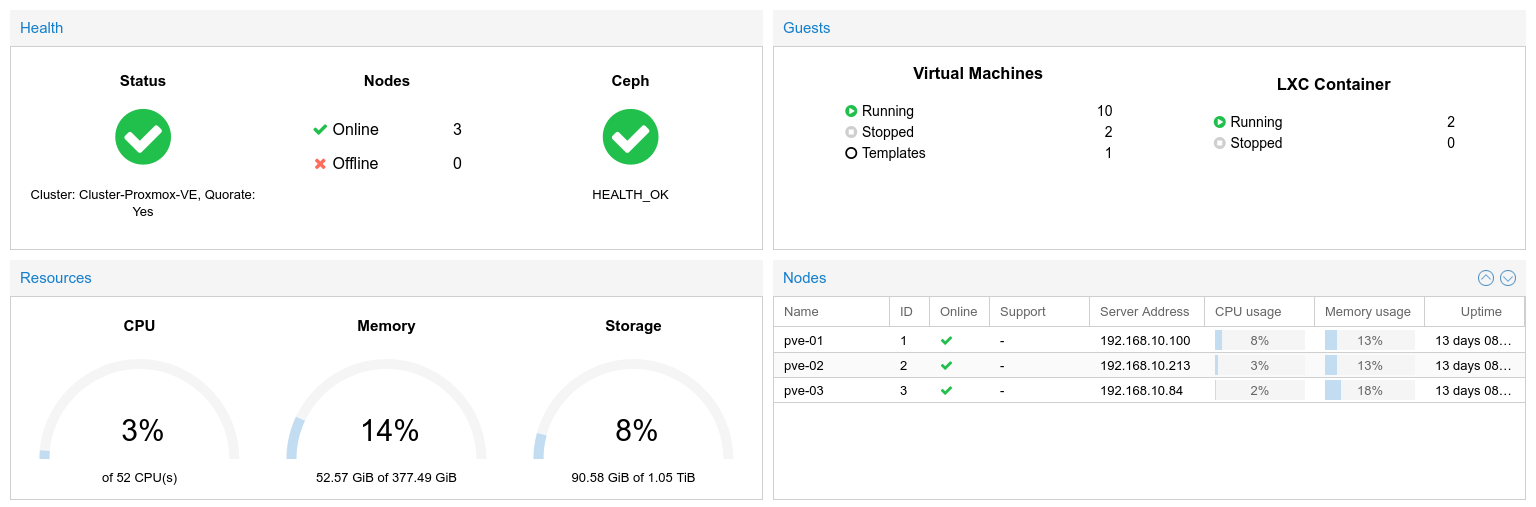
\includegraphics[width=0.9\textwidth]{image/ch4/nodes online.png}
    \caption{Vue du cluster Proxmox montrant les trois nœuds en ligne}
    \label{fig:cluster-three-nodes}
\end{figure}

{\color{bleuuu} \subsubsection{Configuration de la migration à chaud}}

\par La migration à chaud des machines virtuelles a été configurée pour utiliser le réseau dédié VxLAN 50. Ce choix permet de ne pas mélanger le trafic de migration avec le trafic utilisateur ou le trafic de stockage.\\

\par Dans la configuration du datacenter Proxmox, les paramètres de migration ont été ajustés pour utiliser un réseau spécifique et garder un niveau de sécurité acceptable. Une migration manuelle de test a ensuite été réalisée depuis l’interface web afin de vérifier le déplacement transparent d’une VM d’un nœud à un autre sans interruption notable du service.\\

\begin{figure}[H]
    \centering
    
\includegraphics[width=0.9\textwidth]{image/ch4/before migration.png}
    \caption{Avant et après une migration live d’une machine virtuelle}
    \label{fig:live-migration-before-after}
\end{figure}
\begin{figure}[H]
    \centering
    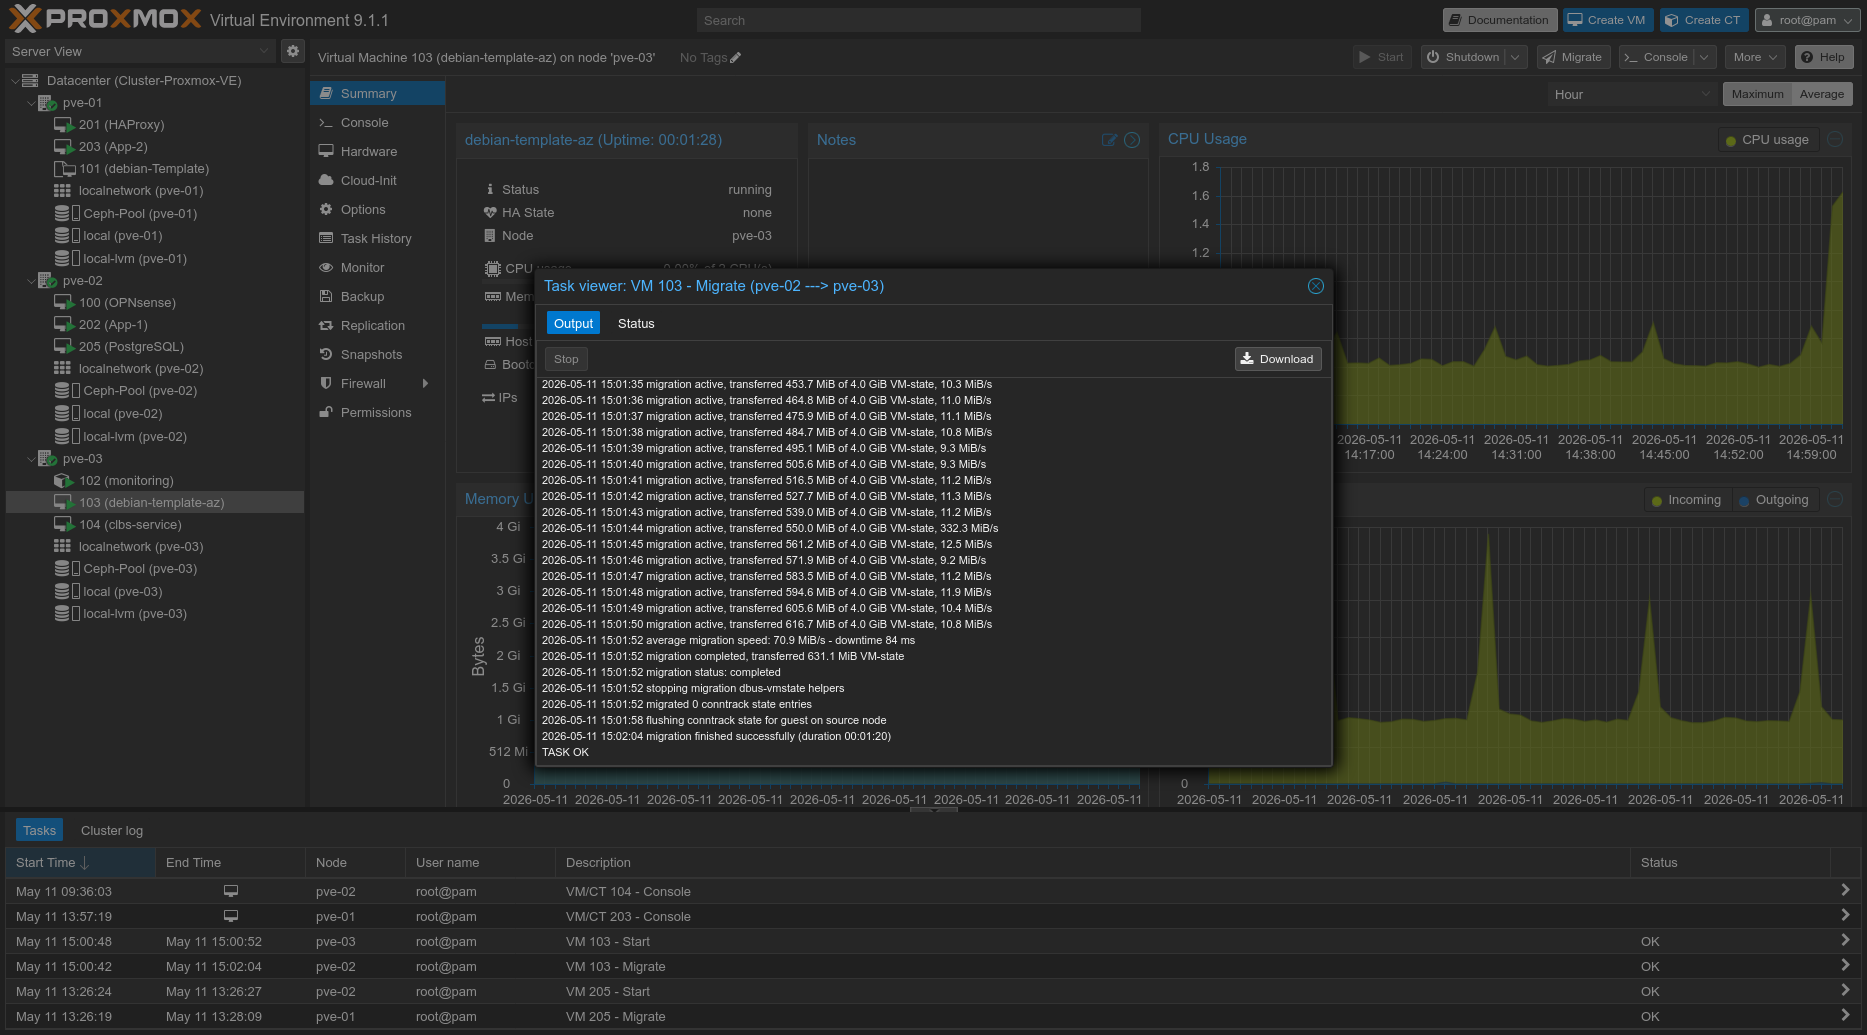
\includegraphics[width=0.9\textwidth]{image/ch4/after migration.png}
    \caption{Avant et après une migration live d’une machine virtuelle}
    \label{fig:live-migration-before-after}
\end{figure}

{\color{bleuu} \subsection{Déploiement de la stack de monitoring}}

\par Afin de superviser l’état global de l’infrastructure, une stack de monitoring a été déployée dans un conteneur LXC dédié appelé \texttt{monitoring}, avec l’adresse \texttt{192.168.10.99}. Ce conteneur centralise InfluxDB, Prometheus et Grafana.\\

{\color{bleuuu} \subsubsection{Déploiement d’InfluxDB}}

\par InfluxDB a été installé pour recevoir les métriques envoyées directement par Proxmox à travers le système natif \textit{Metric Server}. Un bucket nommé \texttt{proxmox-metrics} a été créé afin de stocker les mesures CPU, mémoire, réseau et stockage de chaque nœud du cluster.\\

\par Une fois la configuration validée dans l’interface web Proxmox, les métriques ont commencé à être transmises automatiquement sans agent supplémentaire. La présence des séries temporelles dans l’interface InfluxDB a confirmé le bon fonctionnement de ce mécanisme.\\

\begin{figure}[H]
    \centering
    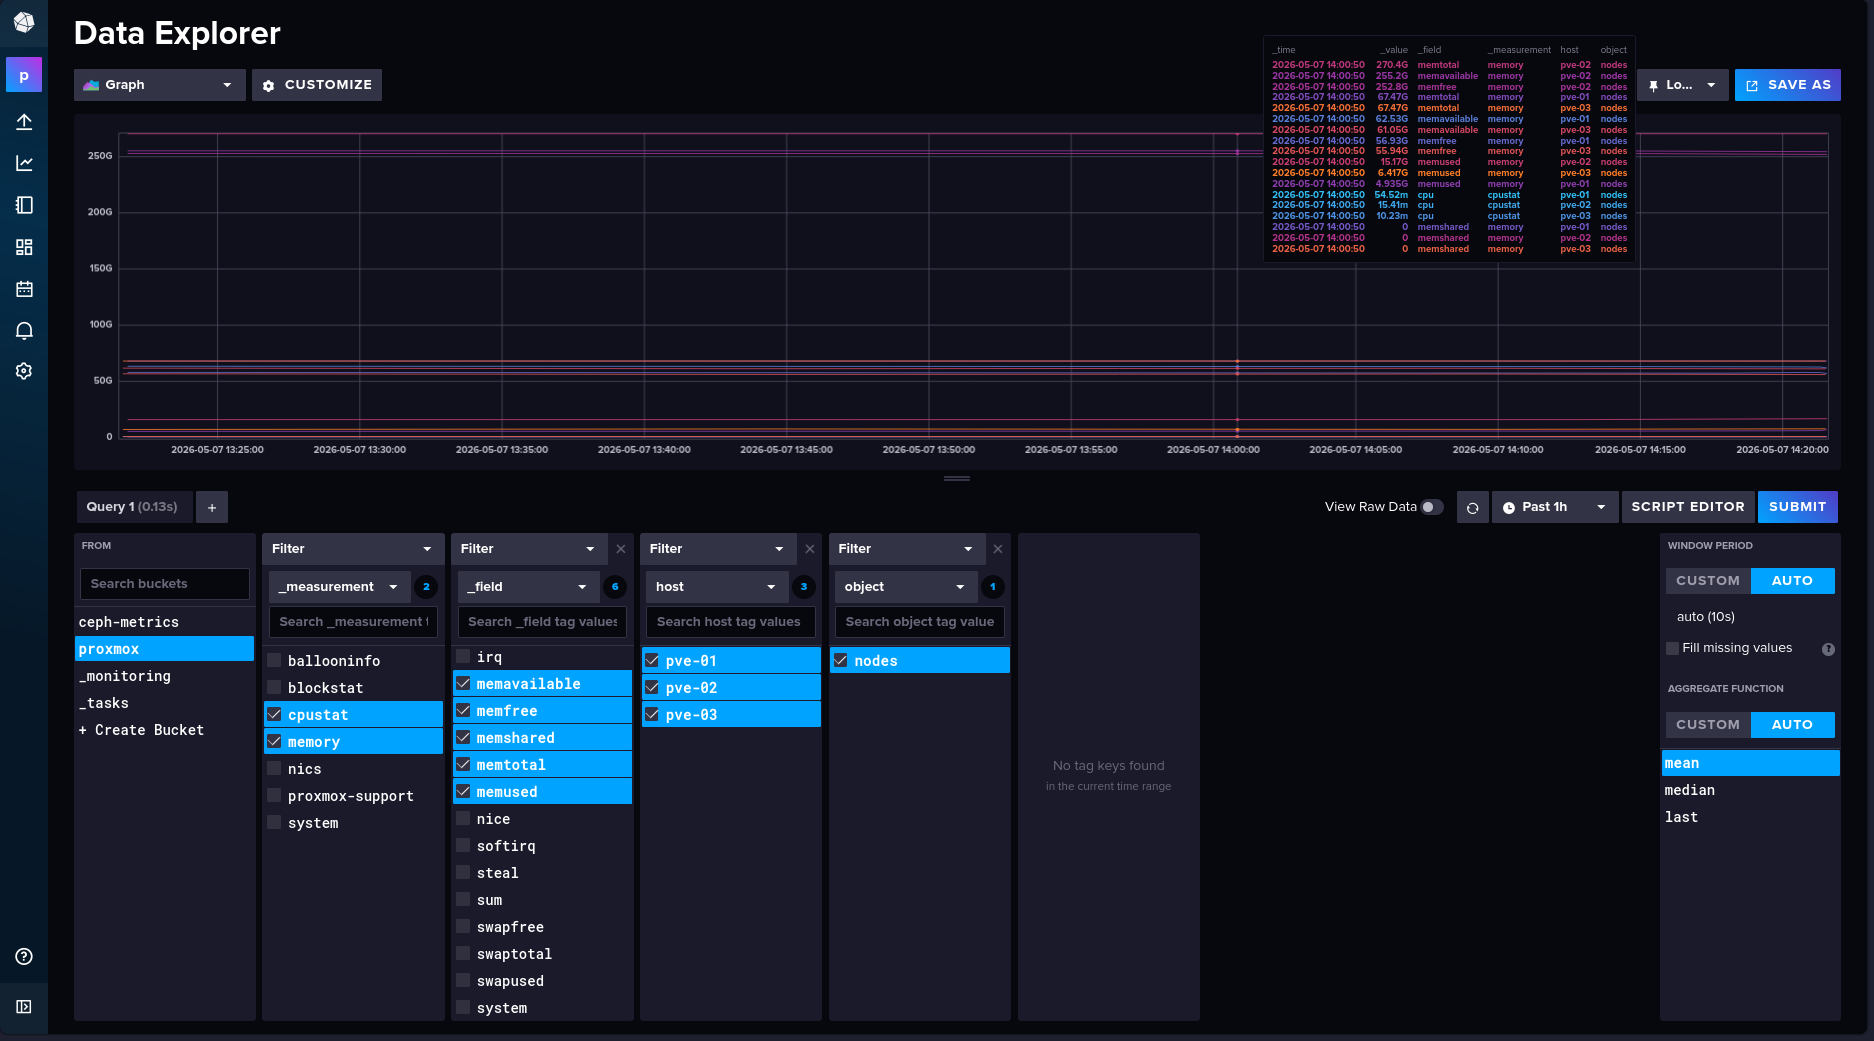
\includegraphics[width=0.9\textwidth]{image/ch4/influxdb.png}
    \caption{Explorateur InfluxDB montrant les métriques reçues depuis Proxmox}
    \label{fig:influxdb-data-explorer}
\end{figure}

{\color{bleuuu} \subsubsection{Déploiement de Prometheus}}

\par Prometheus a été installé dans le même conteneur afin de collecter les métriques exposées par Ceph et par le service applicatif CLBS. La configuration du fichier \texttt{prometheus.yml} contient deux jobs principaux : un job pour les métriques Ceph via le module MGR Prometheus, et un job pour l’application CLBS développée en Go.\\

\begin{lstlisting}[style=sonacode,language=yaml,caption={Extrait du fichier prometheus.yml},label={lst:prometheus-yml}]
global:
  scrape_interval: 30s
  evaluation_interval: 30s

scrape_configs:
  - job_name: ceph
    static_configs:
      - targets:
          - "192.168.10.213:9283"
          - "192.168.10.83:9283"
          - "192.168.10.100:9283"
        labels:
          cluster: "proxmox-lab"

  - job_name: "clbs"
    static_configs:
      - targets: ["192.168.10.104:9101"]
        scrape_interval: 30s
        scrape_timeout: 10s
\end{lstlisting}

\par L’interface web Prometheus a ensuite permis de confirmer que les différentes cibles apparaissaient avec l’état \texttt{UP}.\\

{\color{bleuuu} \subsubsection{Déploiement de Grafana}}

\par Grafana a été ajouté comme couche de visualisation unifiée pour les métriques de Proxmox, Ceph et CLBS. Deux sources de données ont été configurées : InfluxDB pour les métriques de Proxmox, et Prometheus pour les métriques Ceph et applicatives.\\

\begin{table}[H]
\centering
\caption{Dashboards Grafana configurés}
\begin{tabular}{|l|l|l|}
\hline
\textbf{Dashboard} & \textbf{Source} & \textbf{Métriques principales} \\
\hline
Proxmox Cluster & InfluxDB & CPU, RAM, réseau par nœud \\
\hline
Ceph & Prometheus & Santé cluster, pools, latence OSD \\
\hline
CLBS & Prometheus & Historique des migrations \\
\hline
\end{tabular}
\end{table}

\par Trois dashboards principaux ont ainsi été utilisés : un dashboard infrastructure Proxmox, un dashboard Ceph, et un dashboard personnalisé pour le service CLBS.\\

\begin{figure}[H]
    \centering
    \includegraphics[width=0.9\textwidth]{image/ch4/Grafana.png}
    \caption{Dashboard Grafana Infrastructure pour les nœuds Proxmox}
    \label{fig:grafana-proxmox-dashboard}
\end{figure}

{\color{bleuu} \subsection{Implémentation du mécanisme CLBS}}

{\color{bleuuu} \subsubsection{Structure du service}}

\par Le service CLBS (\textit{Cluster Load Balancing Service}) a été développé en langage Go dans une VM dédiée accessible sur le réseau de management. Son rôle est d’analyser périodiquement la charge CPU du cluster et de déclencher automatiquement des migrations live lorsque cela est nécessaire.\\

\par Le code est structuré en plusieurs composants : un lecteur InfluxDB pour les métriques historiques, un client API Proxmox pour piloter le cluster, un calculateur de bandes de charge, et un moteur principal de décision. Les paramètres de connexion sont placés dans un fichier \texttt{.env} chargé au démarrage du service.\\

{\color{bleuuu} \subsubsection{Logique de décision}}

\par À chaque cycle, le service récupère la charge des nœuds, calcule les bornes de charge modérée, puis classe les nœuds dans les catégories \textit{heavy}, \textit{moderate} ou \textit{light}. Si un déséquilibre est détecté entre un nœud surchargé et un nœud léger, le moteur choisit la VM la plus adaptée à migrer.\\

\par Plusieurs mécanismes de protection ont été ajoutés pour éviter les migrations excessives, comme un temps de cooldown global, un cooldown individuel par VM et une suspension temporaire en cas de fréquence de migration trop élevée.\\

{\color{bleuuu} \subsubsection{Déploiement comme service systemd}}

\par Une fois compilé, le binaire Go a été déployé sur la VM CLBS puis intégré comme service \texttt{systemd} afin d’assurer un démarrage automatique et une relance en cas de panne.\\

\begin{lstlisting}[style=sonacode,language=bash,caption={Gestion du service CLBS avec systemd},label={lst:clbs-systemd}]
systemctl enable clbs
systemctl start clbs
journalctl -u clbs.service -f -o cat
\end{lstlisting}

{\color{bleuuu} \subsubsection{Validation du mécanisme}}

\par Pour valider le comportement du service, deux VMs de test ont été créées puis soumises à une charge CPU artificielle avec l’outil \texttt{stress-ng}. Le service CLBS a détecté la surcharge et a déclenché une migration live vers un nœud moins chargé.\\

\begin{lstlisting}[style=sonacode,language=bash,caption={Génération d’une charge CPU de test},label={lst:stress-ng}]
stress-ng --cpu 8
\end{lstlisting}

\begin{figure}[H]
    \centering
    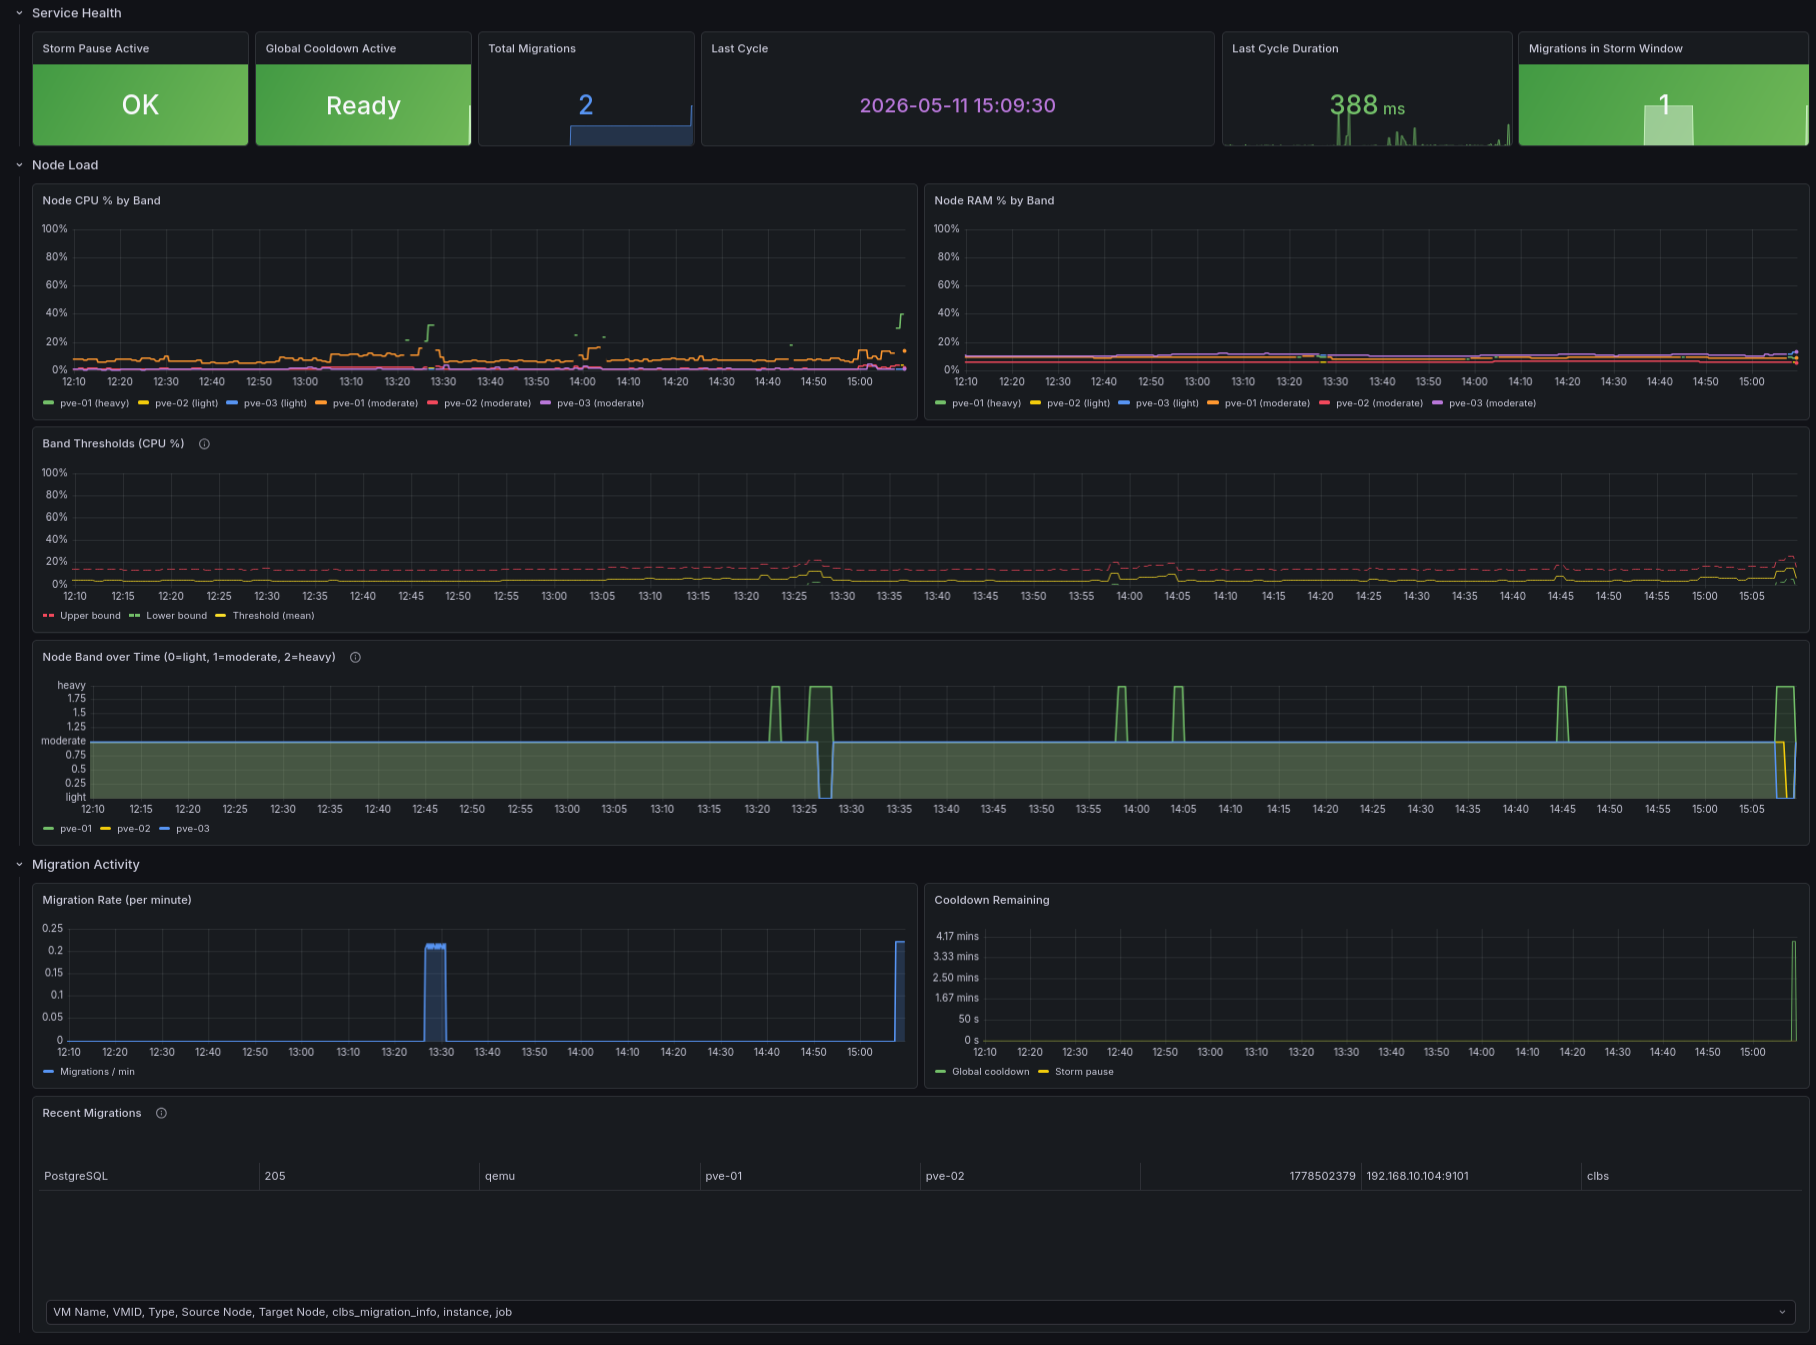
\includegraphics[width=0.9\textwidth]{image/ch4/clbs dashboard.png}
    \caption{Dashboard ou logs montrant une migration déclenchée par CLBS}
    \label{fig:clbs-migration-event}
\end{figure}

{\color{bleuu} \subsection{Déploiement de l’application Sona-Web}}

{\color{bleuuu} \subsubsection{Création des machines virtuelles}}

\par L’application Sona-Web a été déployée sous la forme de plusieurs VMs créées à partir d’un template Debian stocké dans le pool Ceph. Cette architecture comprend une VM HAProxy en frontal, deux VMs Flask pour la couche applicative, et une VM PostgreSQL pour la base de données.\\

\par Les VMs ont été déployées sur les réseaux internes appropriés, avec attribution d’adresse IP par DHCP selon la zone de sécurité visée. Cette organisation permet de séparer la partie exposée, la partie applicative et la base de données.\\

{\color{bleuuu} \subsubsection{Validation de l’application}}

\par La validation a porté sur le fonctionnement du load balancing ainsi que sur la disponibilité de l’application. Des requêtes répétées à travers HAProxy ont montré une alternance correcte entre les serveurs applicatifs Flask, confirmant le bon fonctionnement du mécanisme de répartition de charge.\\

\begin{lstlisting}[style=sonacode,language=bash,caption={Test de répartition HAProxy},label={lst:haproxy-test}]
for i in $(seq 1 10); do
  curl -s http://172.16.80.x | grep "Server"
done
\end{lstlisting}

{\color{bleuu} \subsection{Automatisation avec Ansible}}

{\color{bleuuu} \subsubsection{Environnement et structure du projet}}

\par Afin de simplifier le provisionnement des machines virtuelles et de rendre l’infrastructure plus reproductible, un environnement Ansible a été mis en place. Les connexions se font via SSH depuis les postes des développeurs vers le réseau de management, sans installation d’agent sur les nœuds cibles.\\

\begin{lstlisting}[style=sonacode,language={},caption={Structure du projet Ansible},label={lst:ansible-tree}]
ansible-infra/
├── ansible.cfg
├── secrets.yml
├── inventory/
│   ├── hosts.yml
│   └── proxmox_nodes.yml
└── playbooks/
    ├── provision_vm.yml
    └── provision_vm_batch.yml
\end{lstlisting}

\begin{lstlisting}[style=sonacode,language=ini,caption={Fichier ansible.cfg},label={lst:ansible-cfg}]
[defaults]
inventory            = inventory/hosts.yml
remote_user          = ansible
private_key_file     = ~/.ssh/ansible_ed25519
host_key_checking    = False
interpreter_python   = /usr/bin/python3

[privilege_escalation]
become      = True
become_user = root
\end{lstlisting}

{\color{bleuuu} \subsubsection{Inventaire}}

\par L’inventaire regroupe les nœuds Proxmox, les VMs permanentes, ainsi qu’un groupe dynamique destiné aux nouvelles VMs provisionnées par les playbooks.\\

\begin{lstlisting}[style=sonacode,language=yaml,caption={Extrait de l’inventaire hosts.yml},label={lst:ansible-hosts}]
all:
  children:
    proxmox_nodes:
      hosts:
        pve-01: {ansible_host: 192.168.10.100}
        pve-02: {ansible_host: 192.168.10.213}
        pve-03: {ansible_host: 192.168.10.84}
    vms:
      hosts:
        monitoring:
          ansible_host: 192.168.10.99
    provisioned_vms:
      hosts: {}
\end{lstlisting}

{\color{bleuuu} \subsubsection{Playbook de provisionnement}}

\par Le playbook principal automatise la création d’une VM à partir d’un template Debian déjà préparé. Il configure les ressources matérielles, le réseau, le cloud-init, le démarrage de la VM, puis sa validation après boot.\\

\begin{lstlisting}[style=sonacode,language=bash,caption={Exemple d’utilisation du playbook provision\_vm.yml},label={lst:ansible-vm-create}]
ansible-playbook playbooks/provision_vm.yml \
  -e "vm_id=110 vm_name=web-01"

ansible-playbook playbooks/provision_vm.yml \
  -e "vm_id=115 vm_name=db-01 vm_cores=4 vm_memory=8192"
\end{lstlisting}

\par L’adresse IP de la VM peut être générée automatiquement à partir du VMID pour simplifier le déploiement.\\

\begin{lstlisting}[style=sonacode,language=yaml,caption={Formule d’attribution automatique de l’adresse IP},label={lst:auto-ip-formula}]
vm_ip: "172.16.60.{{ vm_id | int - 90 }}"
\end{lstlisting}

\par La configuration cloud-init repose sur trois commandes successives : attachement du disque cloud-init, injection de la configuration réseau, puis régénération de l’ISO cloud-init.\\

\begin{lstlisting}[style=sonacode,language=bash,caption={Configuration cloud-init d’une VM Proxmox},label={lst:cloud-init-qm}]
qm set {{ vm_id }} --ide2 {{ ceph_pool }}:cloudinit
qm set {{ vm_id }} --ipconfig0 ip={{ vm_cidr }},gw={{ vm_gw }} --nameserver {{ vm_dns }}
qm cloudinit update {{ vm_id }}
\end{lstlisting}

{\color{bleuuu} \subsubsection{Provisionnement en lot et pipeline PXE/TFTP}}

\par Un second playbook permet le provisionnement en lot de plusieurs VMs à partir d’une liste définie à l’avance. En complément, un pipeline PXE/TFTP a été prévu pour automatiser à terme l’installation de nouveaux nœuds physiques Proxmox sans intervention manuelle, ce qui améliore la capacité de montée en charge de la plateforme.\\

{\color{bleu} \section{Partie II --- Couche Stockage}}

{\color{bleuu} \subsection{Déploiement du cluster Ceph}}

{\color{bleuuu} \subsubsection{Initialisation de Ceph}}

\par La couche stockage repose sur un cluster Ceph intégré directement à Proxmox. L’initialisation a été effectuée depuis l’interface web ou via la ligne de commande, en définissant un réseau cluster dédié et un réseau public séparé.\\

\begin{lstlisting}[style=sonacode,language=bash,caption={Initialisation du cluster Ceph},label={lst:ceph-init}]
pveceph init --network 10.10.30.0/24
\end{lstlisting}

\par Le réseau \texttt{10.10.30.0/24} a été réservé aux échanges internes Ceph, tandis que le réseau \texttt{10.10.40.0/24} a été utilisé comme réseau public.\\

{\color{bleuuu} \subsubsection{Déploiement des MON et MGR}}

\par Un moniteur Ceph a été créé sur chaque nœud du cluster afin d’assurer le quorum et la haute disponibilité des métadonnées du cluster.\\

\begin{lstlisting}[style=sonacode,language=bash,caption={Création d’un monitor Ceph},label={lst:ceph-mon-create}]
pveceph mon create
\end{lstlisting}

\par Des managers Ceph ont aussi été déployés pour fournir les fonctions d’administration avancée et l’export des métriques vers Prometheus.\\

\begin{lstlisting}[style=sonacode,language=bash,caption={Activation du module Prometheus pour Ceph},label={lst:ceph-prometheus}]
ceph mgr module enable prometheus
\end{lstlisting}

{\color{bleuuu} \subsubsection{Déploiement des OSDs}}

\par Chaque nœud a reçu un disque dédié transformé en OSD afin de participer au stockage distribué. Le déploiement a été réalisé sur \texttt{/dev/sdb} pour chacun des trois serveurs.\\

\begin{lstlisting}[style=sonacode,language=bash,caption={Création d’un OSD Ceph},label={lst:ceph-osd-create}]
pveceph osd create /dev/sdb
\end{lstlisting}

\par Au total, le cluster dispose de trois OSDs, distribués sur les trois nœuds physiques. La hiérarchie CRUSH a ensuite été vérifiée pour confirmer la bonne prise en compte de tous les nœuds de stockage.\\

\begin{lstlisting}[style=sonacode,language=bash,caption={Affichage de l’arbre CRUSH},label={lst:ceph-osd-tree}]
ceph osd tree
\end{lstlisting}

{\color{bleuuu} \subsubsection{Création du pool de stockage}}

\par Un pool RBD a été créé avec une réplication de taille 3 et une taille minimale de 2, ce qui garantit la disponibilité des données même en cas de perte d’un nœud.\\

\begin{lstlisting}[style=sonacode,language=bash,caption={Création du pool Ceph},label={lst:ceph-pool-create}]
pveceph pool create ceph-pool --size 3 --min-size 2
\end{lstlisting}

\par Ce pool a ensuite été intégré comme stockage partagé dans Proxmox pour héberger les disques des VMs et des conteneurs.\\

\begin{lstlisting}[style=sonacode,language=bash,caption={État global du cluster Ceph},label={lst:ceph-status}]
ceph -s
ceph df
\end{lstlisting}

\begin{figure}[H]
    \centering
    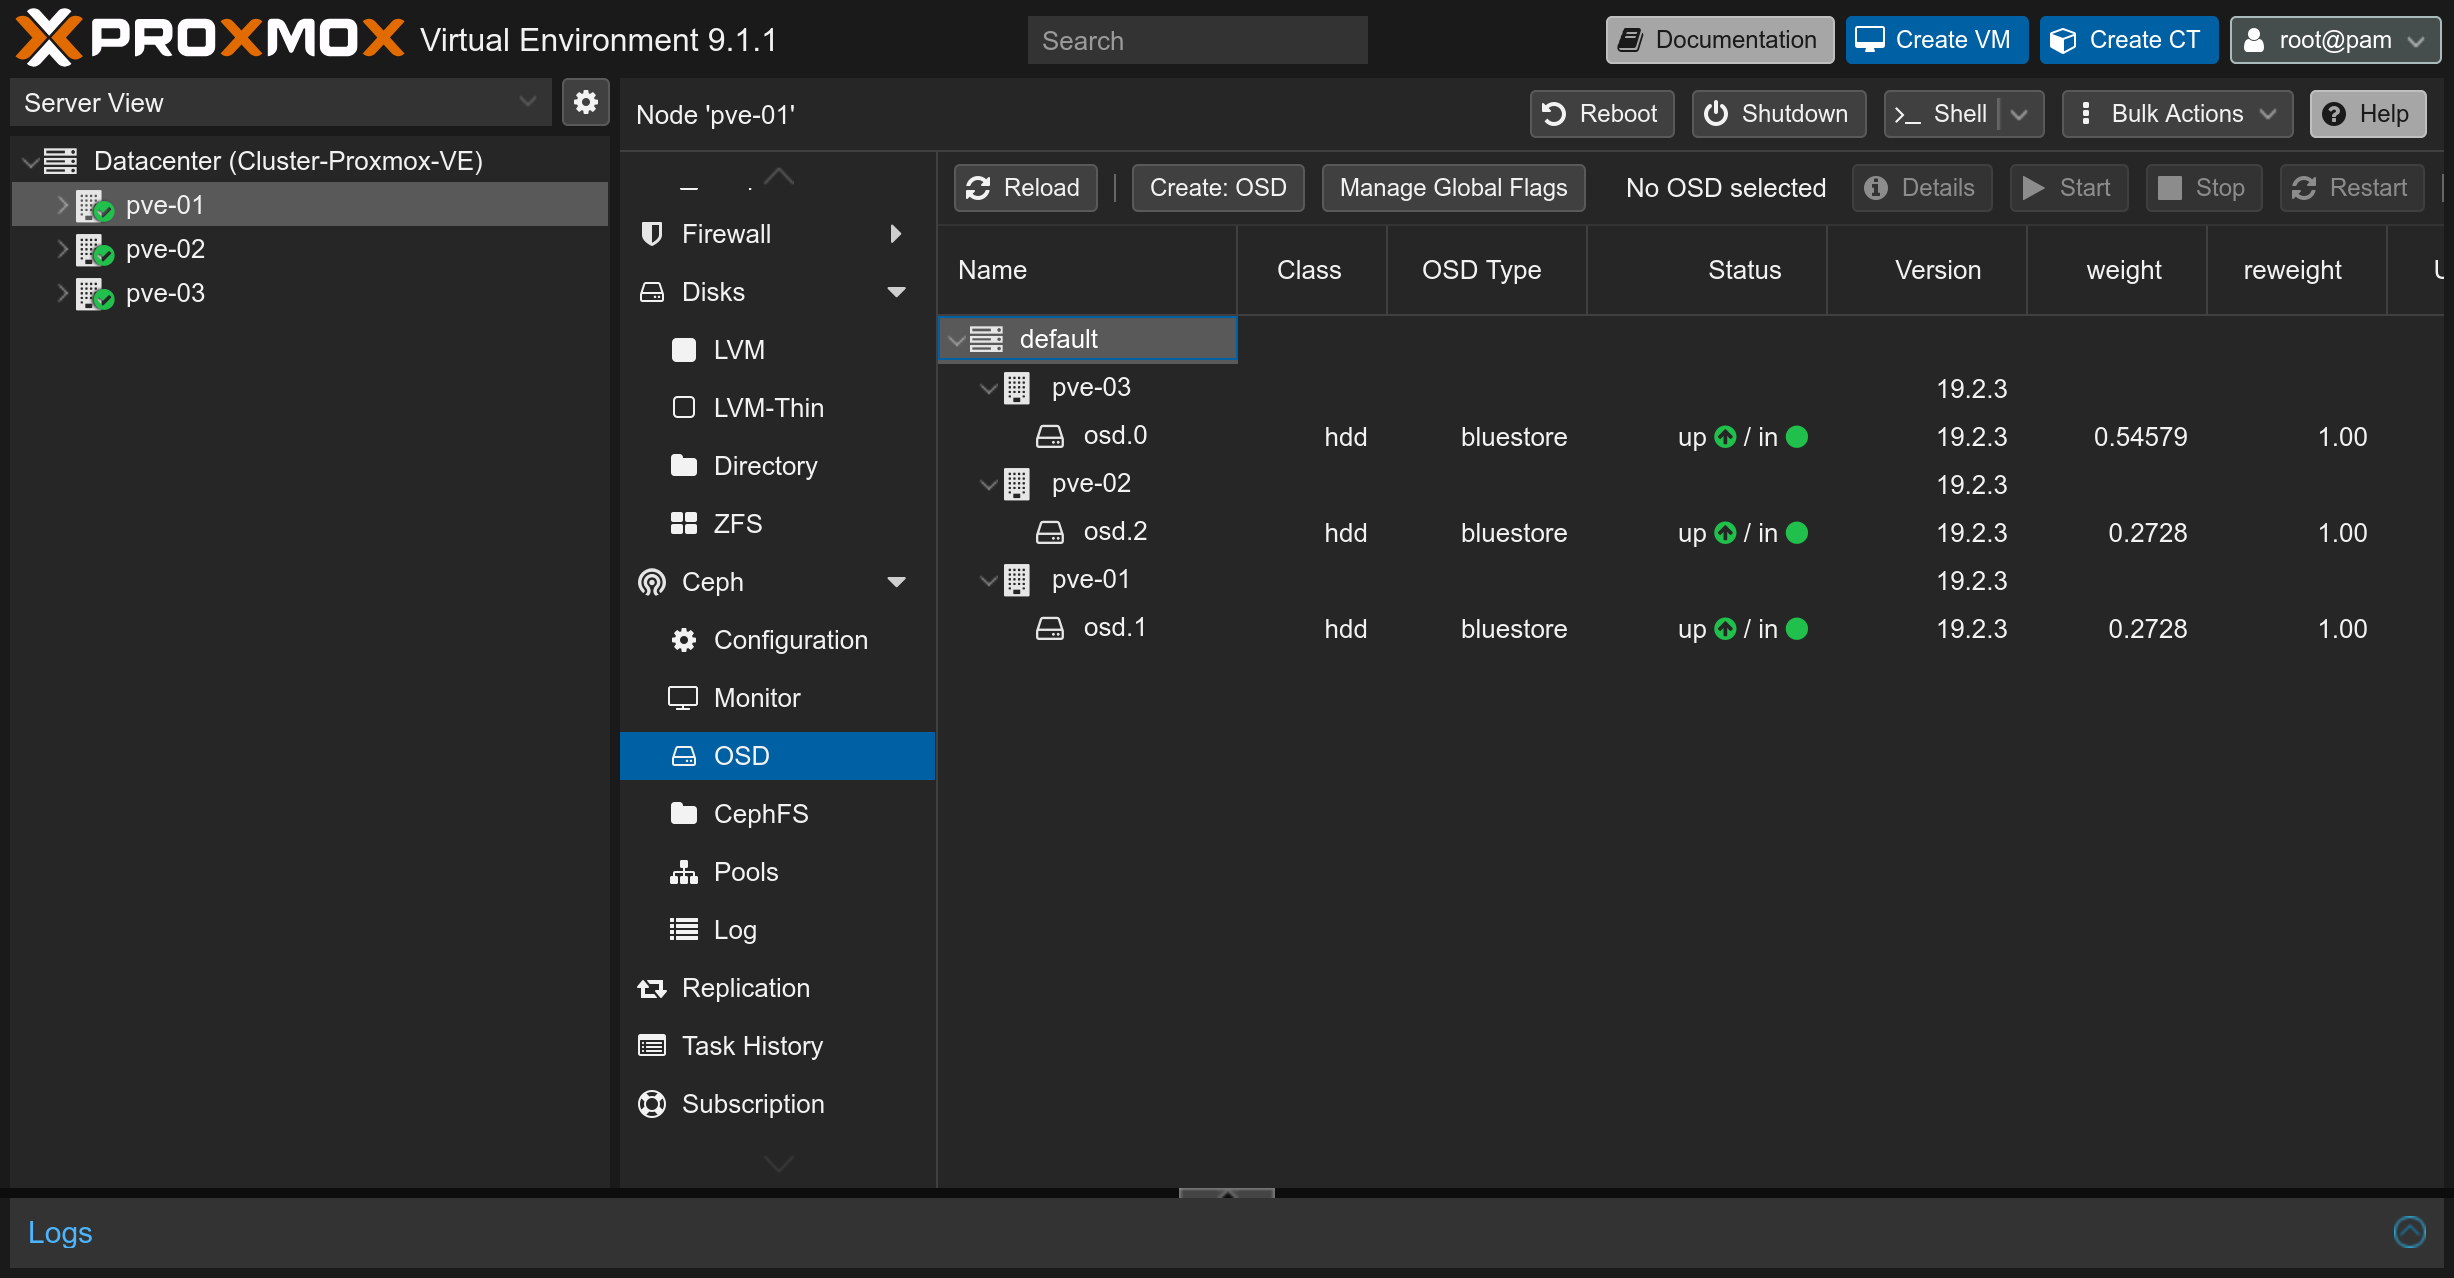
\includegraphics[width=0.9\textwidth]{image/ch4/ceph osd.png}
    \caption{État du cluster Ceph montrant les MON, OSD et le pool RBD}
    \label{fig:ceph-health-ok}
\end{figure}
\begin{figure}[H]
    \centering
    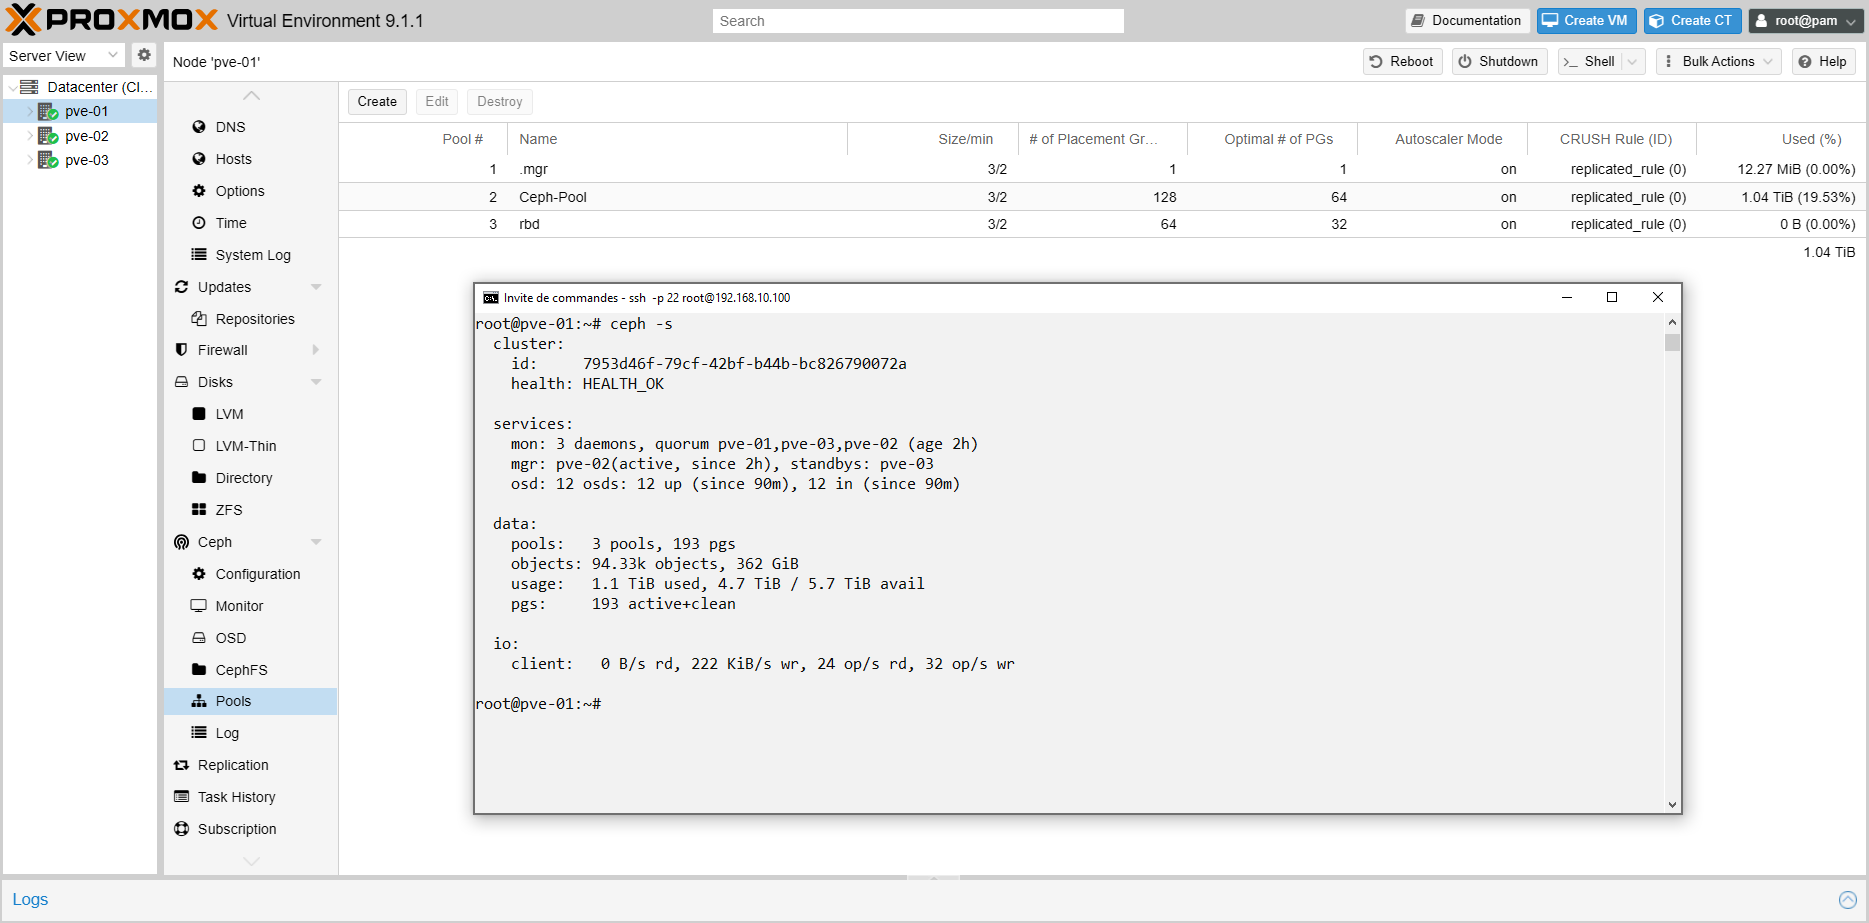
\includegraphics[width=0.9\textwidth]{image/ch4/ceph pool health.png}
    \caption{État du cluster Ceph montrant les MON, OSD et le pool RBD}
    \label{fig:ceph-health-ok}
\end{figure}

{\color{bleuu} \subsection{Validation de la tolérance aux pannes}}

\par La tolérance aux pannes de la couche stockage a été vérifiée par un scénario de panne simulée. Lors de l’extinction d’un nœud, le cluster Ceph est passé temporairement à l’état \texttt{HEALTH\_WARN}, mais les données sont restées accessibles grâce au facteur de réplication.\\

\par Après le retour du nœud défaillant, Ceph a automatiquement lancé la resynchronisation des données et l’état du cluster est revenu à \texttt{HEALTH\_OK}. Ce test valide le bon comportement de la couche stockage distribuée.\\

{\color{bleu} \section{Partie III --- Couche Réseau}}

{\color{bleuu} \subsection{Configuration Open vSwitch et tunnels VxLAN}}

{\color{bleuuu} \subsubsection{Installation d’Open vSwitch}}

\par Open vSwitch a été installé sur chaque nœud Proxmox afin de construire une couche réseau virtuelle flexible, adaptée au transport de plusieurs flux logiques sur le même réseau physique.\\

\begin{lstlisting}[style=sonacode,language=bash,caption={Installation d’Open vSwitch},label={lst:ovs-install}]
apt install openvswitch-switch
\end{lstlisting}

\par Un bridge principal a été créé sur chaque nœud, puis l’interface physique principale y a été attachée pour servir de point de transit à tous les tunnels VxLAN.\\

\begin{lstlisting}[style=sonacode,language=bash,caption={Création du bridge OVS principal},label={lst:ovs-create-bridge}]
ovs-vsctl add-br vmbr1
ovs-vsctl add-port vmbr1 eno1
\end{lstlisting}

{\color{bleuuu} \subsubsection{Configuration complète des interfaces sur PVE-01}}

\par Le fichier \texttt{/etc/network/interfaces} du nœud PVE-01 centralise l’ensemble de la configuration réseau, y compris le bridge principal, les interfaces VXLAN point-à-point vers les autres nœuds, les interfaces internes OVS, et les bridges Linux utilisés pour connecter les machines virtuelles.\\

\begin{lstlisting}[style=sonacode,language={},caption={Configuration réseau complète de PVE-01},label={lst:pve01-full-interfaces}]
auto lo
iface lo inet loopback

iface nic0 inet manual

auto vmbr0
iface vmbr0 inet static
    address 192.168.10.100/24
    gateway 192.168.10.36
    ovs_type OVSBridge
    ovs_ports nic0

auto nic0
iface nic0 inet manual
    ovs_type OVSPort
    ovs_bridge vmbr0

iface nic1 inet manual
iface nic2 inet manual
iface nic3 inet manual

# ===== COROSYNC VXLAN =====
auto vxlan20-pve02
iface vxlan20-pve02 inet manual
    ovs_type OVSPort
    ovs_bridge vmbr0
    ovs_options type=vxlan options:remote_ip=192.168.10.213 options:key=20

auto vxlan20-pve03
iface vxlan20-pve03 inet manual
    ovs_type OVSPort
    ovs_bridge vmbr0
    ovs_options type=vxlan options:remote_ip=192.168.10.84 options:key=20

auto vxlan20-int
iface vxlan20-int inet static
    address 10.10.20.1/24
    ovs_type OVSIntPort
    ovs_bridge vmbr0

# ===== CEPH VXLAN =====
auto vxlan30-pve02
iface vxlan30-pve02 inet manual
    ovs_type OVSPort
    ovs_bridge vmbr0
    ovs_options type=vxlan options:remote_ip=192.168.10.213 options:key=30

auto vxlan30-pve03
iface vxlan30-pve03 inet manual
    ovs_type OVSPort
    ovs_bridge vmbr0
    ovs_options type=vxlan options:remote_ip=192.168.10.84 options:key=30

auto vxlan30-int
iface vxlan30-int inet static
    address 10.10.30.1/24
    ovs_type OVSIntPort
    ovs_bridge vmbr0

# ===== VXLAN 40 (Ceph Public) =====
auto vxlan40-pve02
iface vxlan40-pve02 inet manual
    ovs_type OVSPort
    ovs_bridge vmbr0
    ovs_options type=vxlan options:remote_ip=192.168.10.213 options:key=40

auto vxlan40-pve03
iface vxlan40-pve03 inet manual
    ovs_type OVSPort
    ovs_bridge vmbr0
    ovs_options type=vxlan options:remote_ip=192.168.10.84 options:key=40

auto vxlan40-int
iface vxlan40-int inet static
    address 10.10.40.1/24
    ovs_type OVSIntPort
    ovs_bridge vmbr0

# ===== VXLAN 50 (Migration) =====
auto vxlan50-pve02
iface vxlan50-pve02 inet manual
    ovs_type OVSPort
    ovs_bridge vmbr0
    ovs_options type=vxlan options:remote_ip=192.168.10.213 options:key=50

auto vxlan50-pve03
iface vxlan50-pve03 inet manual
    ovs_type OVSPort
    ovs_bridge vmbr0
    ovs_options type=vxlan options:remote_ip=192.168.10.84 options:key=50

auto vxlan50-int
iface vxlan50-int inet static
    address 10.10.50.1/24
    ovs_type OVSIntPort
    ovs_bridge vmbr0

# ===== VXLAN 90 (Backup) =====
auto vxlan90-pve02
iface vxlan90-pve02 inet manual
    ovs_type OVSPort
    ovs_bridge vmbr0
    ovs_options type=vxlan options:remote_ip=192.168.10.213 options:key=90

auto vxlan90-pve03
iface vxlan90-pve03 inet manual
    ovs_type OVSPort
    ovs_bridge vmbr0
    ovs_options type=vxlan options:remote_ip=192.168.10.84 options:key=90

auto vxlan90-int
iface vxlan90-int inet static
    address 10.10.90.1/24
    ovs_type OVSIntPort
    ovs_bridge vmbr0

# ===== VXLAN 60 =====
auto vxlan60-pve02
iface vxlan60-pve02 inet manual
    ovs_type OVSPort
    ovs_bridge vmbr0
    ovs_options type=vxlan options:remote_ip=192.168.10.213 options:key=60

auto vxlan60-pve03
iface vxlan60-pve03 inet manual
    ovs_type OVSPort
    ovs_bridge vmbr0
    ovs_options type=vxlan options:remote_ip=192.168.10.84 options:key=60

auto vxlan60-int
iface vxlan60-int inet static
    ovs_type OVSIntPort
    ovs_bridge vmbr0

# ===== VXLAN 70 (Dev) =====
auto vxlan70-pve02
iface vxlan70-pve02 inet manual
    ovs_type OVSPort
    ovs_bridge vmbr0
    ovs_options type=vxlan options:remote_ip=192.168.10.213 options:key=70

auto vxlan70-pve03
iface vxlan70-pve03 inet manual
    ovs_type OVSPort
    ovs_bridge vmbr0
    ovs_options type=vxlan options:remote_ip=192.168.10.84 options:key=70

auto vxlan70-int
iface vxlan70-int inet static
    ovs_type OVSIntPort
    ovs_bridge vmbr0

# ===== VXLAN 80 (DMZ) =====
auto vxlan80-pve02
iface vxlan80-pve02 inet manual
    ovs_type OVSPort
    ovs_bridge vmbr0
    ovs_options type=vxlan options:remote_ip=192.168.10.213 options:key=80

auto vxlan80-pve03
iface vxlan80-pve03 inet manual
    ovs_type OVSPort
    ovs_bridge vmbr0
    ovs_options type=vxlan options:remote_ip=192.168.10.84 options:key=80

auto vxlan80-int
iface vxlan80-int inet static
    ovs_type OVSIntPort
    ovs_bridge vmbr0

# ===== VM Bridges =====
auto vmbr60
iface vmbr60 inet manual
    bridge_ports vxlan60-int
    bridge_stp off
    bridge_fd 0

auto vmbr70
iface vmbr70 inet manual
    bridge_ports vxlan70-int
    bridge_stp off
    bridge_fd 0

auto vmbr80
iface vmbr80 inet manual
    bridge_ports vxlan80-int
    bridge_stp off
    bridge_fd 0

source /etc/network/interfaces.d/*
\end{lstlisting}

\par Cette architecture permet de transporter plusieurs réseaux logiques isolés sur le même réseau physique sans dépendre d’un switch physique configuré en VLAN.\\

\begin{table}[H]
\centering
\caption{Résumé des VxLAN utilisés dans l’infrastructure}
\begin{tabular}{|c|l|l|}
\hline
\textbf{VNI} & \textbf{Usage} & \textbf{Réseau} \\
\hline
20 & Corosync / Heartbeat & 10.10.20.0/24 \\
\hline
30 & Ceph Cluster & 10.10.30.0/24 \\
\hline
40 & Ceph Public & 10.10.40.0/24 \\
\hline
50 & Live Migration & 10.10.50.0/24 \\
\hline
60 & Réseau Dev & 172.16.60.0/24 \\
\hline
70 & Réseau Prod & 172.16.70.0/24 \\
\hline
80 & Réseau DMZ & 172.16.80.0/24 \\
\hline
90 & Backup & 10.10.90.0/24 \\
\hline
\end{tabular}
\end{table}

{\color{bleuu} \subsection{Déploiement de la VM OPNsense}}

{\color{bleuuu} \subsubsection{Création et interfaces réseau}}

\par OPNsense a été déployé sous forme de machine virtuelle sur le cluster Proxmox. Son disque système est stocké sur le pool Ceph, ce qui permet de bénéficier du stockage distribué et de la haute disponibilité.\\

\par La VM dispose de 4 Go de RAM, de 2 vCPUs et d’un disque de 20 Go. Quatre interfaces réseau lui ont été attribuées afin de jouer le rôle de routeur et pare-feu pour les différents segments de l’infrastructure.\\

\begin{table}[H]
\centering
\caption{Interfaces de la VM OPNsense}
\begin{tabular}{|l|l|l|l|}
\hline
\textbf{Interface VM} & \textbf{Bridge Proxmox} & \textbf{Rôle} & \textbf{Adresse IP} \\
\hline
net0 (em0) & vmbr0 & WAN & 192.168.10.65/24 \\
\hline
net1 (em1) & vmbr60 & LAN Dev & 172.16.60.1/24 \\
\hline
net2 (em2) & vmbr70 & LAN Prod & 172.16.70.1/24 \\
\hline
net3 (em3) & vmbr80 & LAN DMZ & 172.16.80.1/24 \\
\hline
\end{tabular}
\end{table}

\begin{figure}[H]
    \centering
    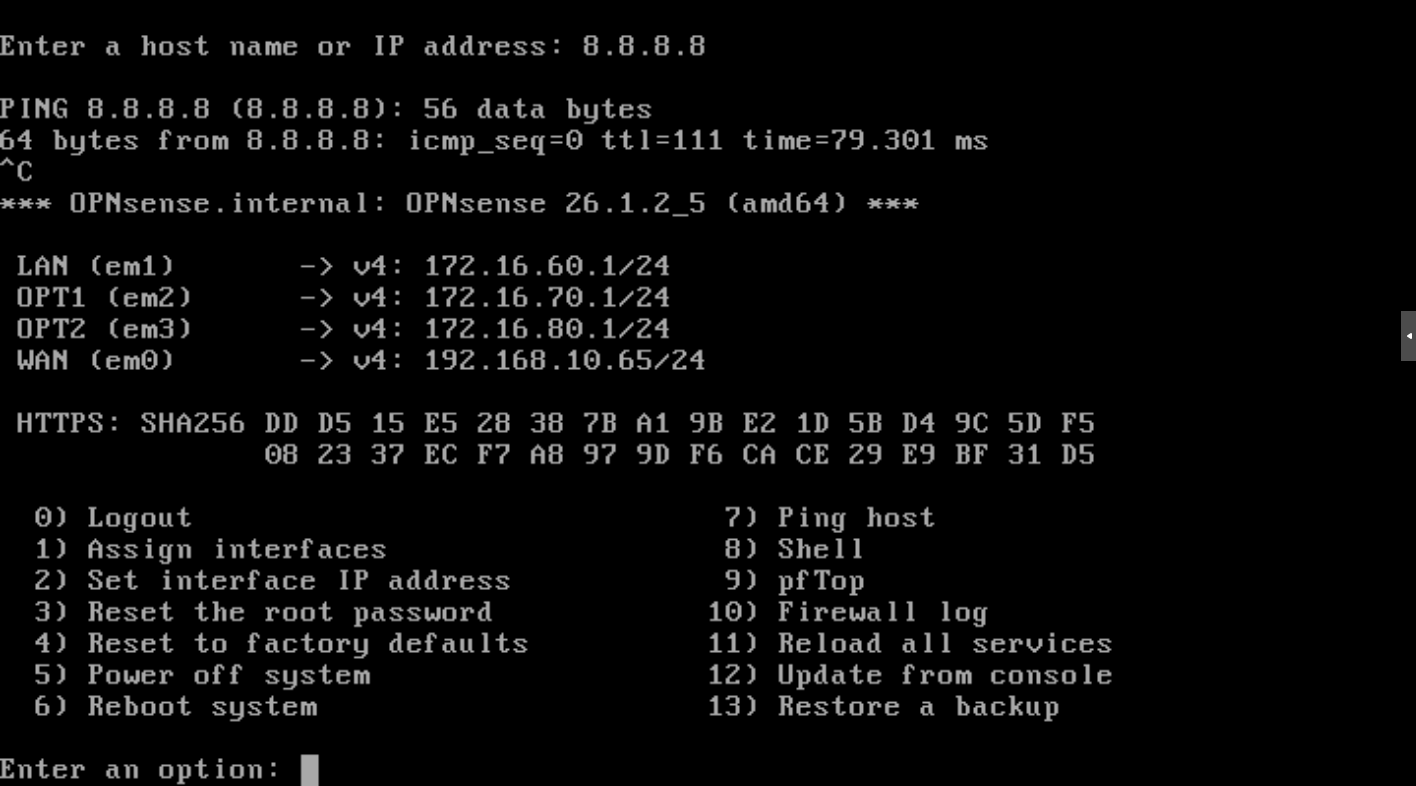
\includegraphics[width=0.9\textwidth]{image/ch4/opnsense.png}
    \caption{Configuration des interfaces de la VM OPNsense}
    \label{fig:opnsense-interfaces}
\end{figure}

{\color{bleuuu} \subsubsection{NAT sortant}}

\par Le NAT sortant automatique a été activé dans OPNsense afin de permettre aux réseaux internes de sortir vers Internet via l’interface WAN. Cette configuration a simplifié le routage pour les VMs hébergées sur les réseaux Dev, Prod et DMZ.\\

{\color{bleuu} \subsection{Configuration du service DHCP}}

\par Le service DHCP a été activé via \texttt{dnsmasq} sur les interfaces LAN internes. Ce choix a été retenu car il est simple à configurer et convient bien à un environnement de laboratoire.\\

\begin{table}[H]
\centering
\caption{Plages DHCP configurées sur OPNsense}
\begin{tabular}{|l|l|l|l|}
\hline
\textbf{Interface} & \textbf{Plage début} & \textbf{Plage fin} & \textbf{Gateway} \\
\hline
LAN (Dev) & 172.16.60.10 & 172.16.60.250 & 172.16.60.1 \\
\hline
OPT1 (Prod) & 172.16.70.10 & 172.16.70.250 & 172.16.70.1 \\
\hline
OPT2 (DMZ) & 172.16.80.10 & 172.16.80.250 & 172.16.80.1 \\
\hline
\end{tabular}
\end{table}

\par Le bon fonctionnement de DHCP a été vérifié par une capture réseau sur l’interface LAN d’OPNsense pendant le démarrage d’une VM de test.\\

\begin{lstlisting}[style=sonacode,language=bash,caption={Capture du trafic DHCP avec tcpdump},label={lst:tcpdump-dhcp}]
tcpdump -i em1 port 67 or port 68
\end{lstlisting}

\par Cette vérification a montré le cycle normal des échanges DHCP, depuis le \textit{Discover} jusqu’au \textit{Offer}, puis l’attribution effective de l’adresse IP à la machine virtuelle.\\

{\color{bleuu} \subsection{Validation de la haute disponibilité réseau et applicative}}

\par Un scénario de panne a été réalisé afin de tester le comportement global de l’infrastructure en cas de perte d’un nœud physique. L’arrêt brutal de PVE-01 a permis d’observer la détection de panne par Corosync, le redémarrage des services protégés sur un autre nœud, puis la resynchronisation automatique après le retour du serveur.\\

\par Cette séquence a montré que le cluster restait opérationnel malgré la défaillance, et que les mécanismes de haute disponibilité répondaient correctement à ce type d’événement.\\

\begin{figure}[H]
    \centering
    \fbox{\rule{0pt}{6cm}\rule{0.9\textwidth}{0pt}}
    \caption{Chronologie des événements lors d’une panne d’un nœud physique}
    \label{fig:ha-failure-sequence}
\end{figure}

{\color{bleu} \section{Conclusion}}

\par Ce chapitre a présenté l’implémentation réelle de l’infrastructure hyperconvergée open source mise en place dans le cadre du projet. La couche calcul a permis de déployer Proxmox, le cluster, le monitoring, l’automatisation et les services applicatifs. La couche stockage a été assurée par Ceph avec réplication et tolérance aux pannes. Enfin, la couche réseau a été construite avec Open vSwitch, les tunnels VxLAN, OPNsense et les services d’adressage associés.\\

\par Les différents tests réalisés ont confirmé la cohérence de l’architecture proposée et sa capacité à répondre aux objectifs du projet dans un environnement de laboratoire structuré. Le chapitre suivant présentera l’évaluation des performances obtenues ainsi qu’une analyse des résultats expérimentaux.\\